\section{Theorie}
\label{sec:Theorie}
Brückenschaltungen werden in der Messtechnik 
eingesetzt um die Auflösung einer Messung zu erhöhen
oder eine pysikalische Größe,
die sich als elektrischer Widerstand darstellen lässt,
zu bestimmen. \\
\\
Dafür muss eine Abgleichbedingung der
Brückenschaltung erfüllt sein. Generell benötigt eine
Brückenschaltung eine Speisespannung $U_s$, den zu
ermittelnden elektrischen Widerstand und bekannte
elektrische Bauteile um ein Widerstandsverhältnis
zu bestimmen.
Die Abgleichbedingung besteht darin, dass die
Brückenspannung $U_Br$ zwischen zwei Punkten
verschwindet.

\begin{figure}[H]
\centering
    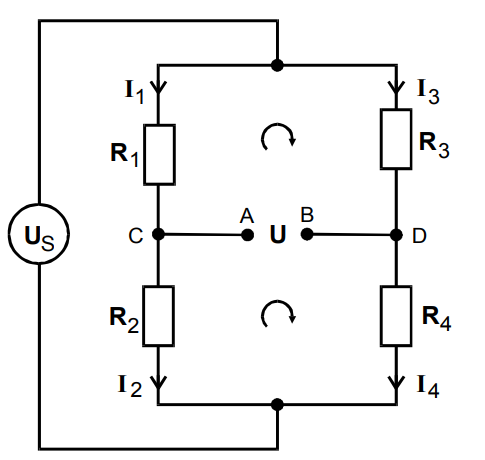
\includegraphics[height= 5cm]{content/Allgemein.png}
\end{figure}

\noindent Ist die Abgleichbedingung erfüllt kann aus dem
Widerstandsverhältnis der unbekannte Widerstand
bestimmt werden.\\
\\
Dieses



\subsection{Wheatstonesche Brücke}
\subsection{Kapazitätsmessbrücke}
\subsection{Induktivitätsmessbrücke}
\subsection{Maxwell-Brücke}
\subsection{Wien-Robinson-Brücke}
\subsection{Fehlerrechnung}
Bei der Auswertung werden die Mittelwerte 
der errechneten Größen durch die Formel
\begin{equation}
    \bar{x}=\frac{1}{N}\sum_{i=1}^N x_i
\end{equation}
berechnet.\\ 
\\
Der Standardfehler des Mittelwerts beerechnet sich durch

 \begin{equation}
     \Delta\bar{x}=\sqrt{\frac{1}{N(N-1)}\sum_{i=1}^N (x_i-\bar{x})}.
 \end{equation}
